\documentclass[]{article}
\usepackage[brazil]{babel}
\usepackage{graphicx}
\usepackage{mathtools}
\usepackage{float} 

\usepackage{array}
\usepackage{booktabs}



% margenes
\usepackage[a4paper,left=3cm,right=3cm,top=3cm]{geometry}

%opening
\title{}
\author{}

\begin{document}

\begin{center}
	{\tiny {\normalsize {\large Lista de exercicios 2 \\
Transferência de calor e mecânica dos fluidos computacional I\\
\textbf{Cristian Herledy Lopez Lara}}}}
\end{center}



\section*{Exercício 3.3}
\subsubsection*{A - Mostrando a expreçao 3.143}

\begin{equation}
	f_{i+1}=f(x_{i}) + \Delta xf'i +\frac{\Delta x^{2}}{2}f''(x_{i}) + \frac{\Delta x^{3}}{3!}f'''(x_{i}) + \frac{\Delta x^{4}}{4!}f^{4}(x_{i})+ O(\Delta x^{5})
\end{equation}

\begin{equation}
f_{i+1}=f(x_{i}) - \Delta xf'i +\frac{\Delta x^{2}}{2}f''(x_{i}) - \frac{\Delta x^{3}}{3!}f'''(x_{i}) + \frac{\Delta x^{4}}{4!}f^{4}(x_{i})- O(\Delta x^{5})
\end{equation}

\begin{equation}
	f_{i+2}=f(x_{i}) + 2\Delta xf'i +\frac{(2\Delta x)^{2}}{2}f''(x_{i}) + \frac{(2\Delta x)^{3}}{3!}f'''(x_{i}) + \frac{(2\Delta x)^{4}}{4!}f^{4}(x_{i})+ O(2\Delta x)^{5}
\end{equation}

\begin{equation}
	f_{i-2}=f(x_{i}) - 2\Delta xf'i +\frac{(2\Delta x)^{2}}{2}f''(x_{i}) - \frac{(2\Delta x)^{3}}{3!}f'''(x_{i}) + \frac{(2\Delta x)^{4}}{4!}f^{4}(x_{i})- O(2\Delta x)^{5}
\end{equation}

\begin{equation}
	f_{i+3}=f(x_{i}) + 3\Delta xf'i +\frac{(2\Delta x)^{3}}{2}f''(x_{i}) + \frac{(3\Delta x)^{3}}{3!}f'''(x_{i}) + \frac{(3\Delta x)^{4}}{4!}f^{4}(x_{i})+ O(3\Delta x)^{5}
\end{equation}

\begin{equation}
	f_{i-3}=f(x_{i}) - 3\Delta xf'i +\frac{(2\Delta x)^{3}}{2}f''(x_{i}) - \frac{(3\Delta x)^{3}}{3!}f'''(x_{i}) + \frac{(3\Delta x)^{4}}{4!}f^{4}(x_{i}) - O(3\Delta x)^{5}
\end{equation}\\
\\
Fazendo um sistema de equações para encontrar os coeficientes que vão para cada termo, as equações 1,3 e 5 ficam assim:

\begin{equation}
	f_{i+1}=f(x_{i}) + A + B + C + D + O(\Delta x^{5})
\end{equation}


\begin{equation}
	f_{i+2}=f(x_{i}) + 2A + 4B + 8C + 16D + O(\Delta x^{5})
\end{equation}

\begin{equation}
	f_{i+3}=f(x_{i}) + 3A + 9B + 27C + 81D + O(\Delta x^{5})
\end{equation}\\

\begin{flushleft}
	Agora multiplicando a equação (7) por -5, a equação (8) por 4 e a equação (9) por -1 obtemos
\end{flushleft}

\begin{equation}
	-5f_{i+1} + 4f_{i+2} -f_{i-3} = -2f_i +\frac{\Delta x^{2}}{2}f''(x_{i})- O(\Delta x)^{4}
\end{equation}\\

Reorganizando\\

\begin{equation}
	\frac{-5f_{i+1} + 4f_{i+2} -f_{i-3} + 2f_i}{\Delta x^{2}} +  O(\Delta x)^{2} = f''(x_{i})
\end{equation}\\

\subsubsection*{B - Mostrando a expreçao 3.144}
Da mesma forma, construindo um sistema de equações usando as equações usando 8(1), -8(2),-(3) e (4):\\

\begin{equation}
	8f_{i+1}=8f(x_{i}) + 8A + 8B + 8C + 8D + 8O(\Delta x^{5})
\end{equation}

\begin{equation}
	-8f_{i-1}=-8f(x_{i}) + 8A - 8B + 8C - 8D + 8O(\Delta x^{5})
\end{equation}

\begin{equation}
	-f_{i+2}=-f(x_{i}) - 2A - 4B - 8C - 16D - 32O(\Delta x^{5})
\end{equation}
\begin{equation}
	f_{i-2}=f(x_{i}) - 2A + 4B - 8C + 16D + 32O(\Delta x^{5})
\end{equation}
Somando as equações obtemos

\begin{equation}
	8f_{i+1} - 8f_{i-1} - f_{i+2} + f_{i-2}  = 12\Delta xf'(x_{i}) - O(\Delta x)^{4}
\end{equation}\\
\begin{equation}
	\frac{8f_{i+1} - 8f_{i-1} - f_{i+2} + f_{i-2}}{12\Delta x} + O(\Delta x)^{4}  = f'(x_{i}) 
\end{equation}\\

\subsubsection*{C - Mostrando a expreçao 3.145}


Calculando a expansão de Taylor

\begin{equation}
f_{i+1, j+1} = f_{i,j} + \Delta x  f'(x_{i}) + \Delta y f'(y_{j}) + \Delta x \Delta y f''(x_{i})(y_{j}) +  O(\Delta x^{3} \Delta y^{3})
\end{equation}

\begin{equation}
	-f_{i+1, j-1} = -f_{i,j} + \Delta x  f'(x_{i}) - \Delta y f'(y_{j}) + \Delta x \Delta y f''(x_{i})(y_{j}) +  O(\Delta x^{3} \Delta y^{3})
\end{equation}

\begin{equation}
	-f_{i-1, j+1} = -f_{i,j} - \Delta x  f'(x_{i}) + \Delta y f'(y_{j}) + \Delta x \Delta y f''(x_{i})(y_{j}) +  O(\Delta x^{3} \Delta y^{3})
\end{equation}

\begin{equation}
	f_{i-1, j-1} = f_{i,j} - \Delta x  f'(x_{i}) - \Delta y f'(y_{j}) + \Delta x \Delta y f''(x_{i})(y_{j}) +  O(\Delta x^{3} \Delta y^{3})
\end{equation}


Somando as equações obtemos 

\begin{equation}
	f_{i+1, j+1} - f_{i+1, j-1} - f_{i-1, j+1} + f_{i-1, j-1} = 4 \Delta x \Delta y f''(x_{i})(y_{j}) + \mathcal{O}(\Delta x^3, \Delta y^3)
\end{equation}

\begin{equation}
	\frac{f_{i+1, j+1} - f_{i+1, j-1} - f_{i-1, j+1} + f_{i-1, j-1}}{4 \Delta x \Delta y} + \mathcal{O}(\Delta x^3, \Delta y^3) =  f''(x_{i})(y_{i})
\end{equation}

\section*{Exercício 3.4}

A equação de condução sendo transiente unidimensional 3.132

\begin{equation}
	\frac{\partial T}{\partial t} = \alpha\frac{\partial^{2} T}{\partial x^{2}}
\end{equation}
Usando diferenças finitas, é discretizada om função de interpolação no tempo
	
\begin{equation}
	T^\theta = \theta T + (1 - \theta) T^o
\end{equation}

\begin{equation}
	\frac{\Delta x T_P}{\Delta t} =
	\frac{a_e}{\Delta x_e} \left[ \theta T_E + (1 - \theta) T_E^0 \right] +
	\frac{a_w}{\Delta x_w} \left[ \theta T_W + (1 - \theta) T_W^0 \right] -
	\left( \frac{a_e}{\Delta x_e} + \frac{a_w}{\Delta x_w} \right) \left[ \theta T_P + (1 - \theta) T_P^0 \right] +
	\frac{T_P^0 \Delta x}{\Delta t}
\end{equation}


Fica

\begin{align*}
	\left( A_P^0 + A_e \theta + A_w \theta \right) T_P &=
	A_e \theta T_E + A_w \theta T_W + A_e (1 - \theta) T_E^0 + A_w (1 - \theta) T_W^0 \\
	&\quad + \left[ -A_e (1 - \theta) - A_w (1 - \theta) + A_P^0 \right] T_P^0
\end{align*}


Fazendo uso do critério de estabilidade de Von Neumann (Livro de Anderson 1984, páginas 84-96)

\begin{equation}
	A_P^0 (T_P - T_P^0) + A_e T_P^\theta + A_w T_P^\theta = A_e T_E^\theta + A_w T_W^\theta
\end{equation}

\begin{equation}
	(T_P - T_P^0) = \frac{A_e T_E^\theta + A_w T_W^\theta - (A_e + A_w) T_P^\theta}{A_P^0}
\end{equation}
Suistituindo

\begin{align*}
	\Delta x_e = \Delta x_w = \Delta x \\ A_e = A_w  \\
	A_e = \frac{1}{\Delta x} \\
	A_w = \frac{1}{\Delta x} \\
	A_P^0 = \frac{\Delta x}{\Delta t}
\end{align*}

\begin{equation}
	(T_P - T_P^0) = \frac{a \Delta t}{\Delta x^2} T_E^\theta + \frac{a \Delta t}{\Delta x^2} T_W^\theta - \frac{2a \Delta t}{\Delta x^2} T_P^\theta
\end{equation}

\begin{equation}
	(T_P - T_P^0) = r (T_E^\theta + T_W^\theta - 2T_P^\theta)
\end{equation}
Donde $r = \alpha\dfrac{\Delta t}{\Delta x^{2}}$ (Ecq 3.24 livro Maliska)

A solução pode ser levada a erros de aproximação por $N = D = \epsilon$

\begin{equation}
	\theta \epsilon_P + (1 - \theta) \epsilon_P^0 - \epsilon_P^0 =
	r \left[ \theta \epsilon_E + (1 - \theta) \epsilon_E^0 + \theta \epsilon_W + (1 - \theta) \epsilon_W^0 - 2 \theta \epsilon_P - 2 (1 - \theta) \epsilon_P^0 \right]
\end{equation}


\begin{equation}
	\epsilon_m(x, t) = e^{a t} e^{i k_m x}
\end{equation}
\begin{equation}
	\epsilon_P = e^{a (t + \Delta t)} e^{i k_m x}
\end{equation}
\begin{equation}
	\epsilon_P^0 = e^{a t} e^{i k_m x}
\end{equation}
\begin{equation}
	\epsilon_E = e^{a (t + \Delta t)} e^{i k_m (x + \Delta x)}
\end{equation}
\begin{equation}
	\epsilon_E^0 = e^{a t} e^{i k_m (x + \Delta x)}
\end{equation}
\begin{equation}
	\epsilon_W = e^{a (t + \Delta t)} e^{i k_m (x - \Delta x)}
\end{equation}
\begin{equation}
	\epsilon_W^0 = e^{a t} e^{i k_m (x - \Delta x)}
\end{equation}

Sustituindo
\begin{equation}
	e^{a \Delta t} = \frac{-1 + 2\theta \cos(i k_m) - 2r \cos(i k_m) + 2r - 2r \theta}{2r \cos(i k_m) - 2r \theta - 1}
\end{equation}

\begin{equation}
	e^{a \Delta t} = \frac{-1 + 2r (\theta - 1) (\cos(i k_m) - 1)}{-1 + 2r \theta (\cos(i k_m) - 1)}
\end{equation}

\begin{equation}
	e^{a \Delta t} = 1 - \frac{2r (\cos(i k_m) - 1)}{2r \theta (\cos(i k_m) - 1) - 1}
\end{equation}

\begin{equation}
	e^{a \Delta t} = 1 - \frac{4r\sin^2\left(\frac{i k_m}{2}\right)}{4r \theta \sin^2\left(\frac{i k_m}{2}\right) + 1}
\end{equation}

\begin{equation}
	 1 - \frac{4r}{4r \theta s + 1}  \leq 1
\end{equation}

\begin{equation}
	\frac{\alpha \Delta t}{\Delta x^2} \leq \frac{1}{2 - 4\theta} \quad ; \theta \leq 0.5
\end{equation}


\begin{equation}
	\frac{\alpha \Delta t}{\Delta x^2} \leq \infty \quad ; 0.5 < \theta \leq 1
\end{equation}






\section*{Exercício 3.6}
A equação de condução sendo transiente unidimensional

\begin{equation}
	\frac{\partial T}{\partial t} = \frac{\partial^{2} T}{\partial x^{2}}
\end{equation}

\begin{flushleft}
	Após integração espacial e temporal e pronto para uma formulação explícita, fica:
\end{flushleft}

\begin{equation}
A_pT_p = AeT_E^{0} + AwT_W^{0} + (A_p^{0}- Ae - Aw)T_p^{0}
\end{equation}\\

Onde 
\begin{equation}
	T_p = (1-2r) T_p^{0} + r T_E^{0} + rT_W^{0}  ;  r = \dfrac{\alpha \Delta t}{\Delta x^{2}} = \Delta t
\end{equation}
Implementando as condições de contorno e iniciais, a evolução da temperatura ao longo do tempo para diferentes discretizações temporais é mostrada abaixo.



\begin{figure}[h]
	\centering
	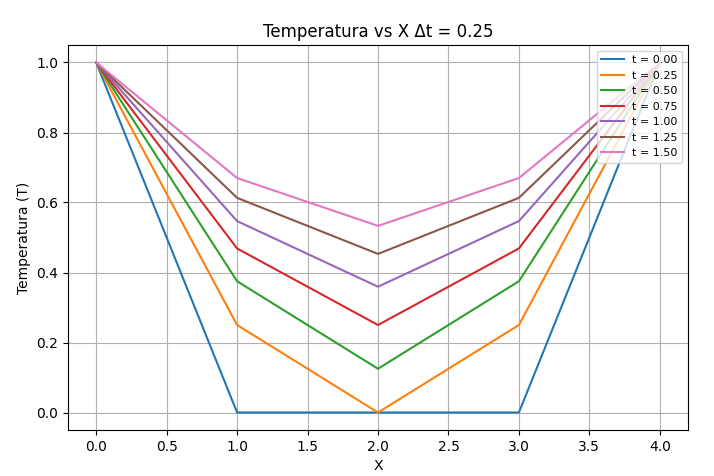
\includegraphics[width=.65\textwidth]{figures/36-1}
	\caption{Temperatura para r=0.25}
\end{figure}

Pode-se observar que a temperatura evolui uniformemente com o avanço do tempo, e para cada ponto espacial existe apenas um valor de temperatura em cada $\Delta t$ Esta evolução é a esperada de um problema real transiente, e está de acordo com a condição de positividade do coeficiente para $T_p^{0}$.

\begin{figure}[h]
	\centering
	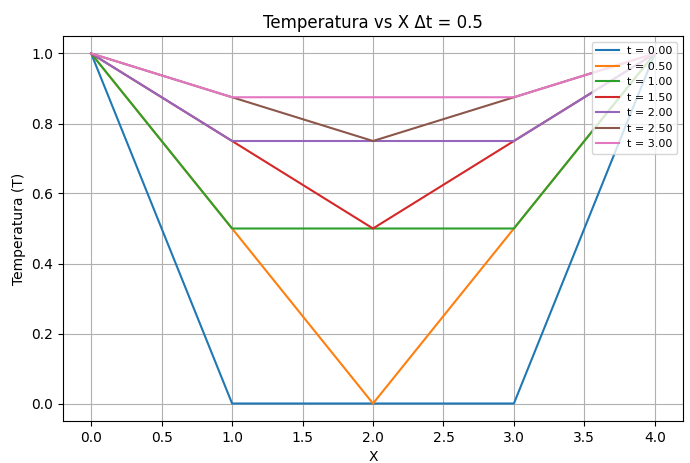
\includegraphics[width=.65\textwidth]{figures/36-2}
	\caption{Temperatura para r=0.5}
\end{figure}

O valor de r próximo de $\frac{1}{2}$ mostra sinais de divergência da solução. Valores T compartilhados são evidentes em vários intervalos de tempo em $x=1$ e $x=3$.

\begin{figure}[h]
	\centering
	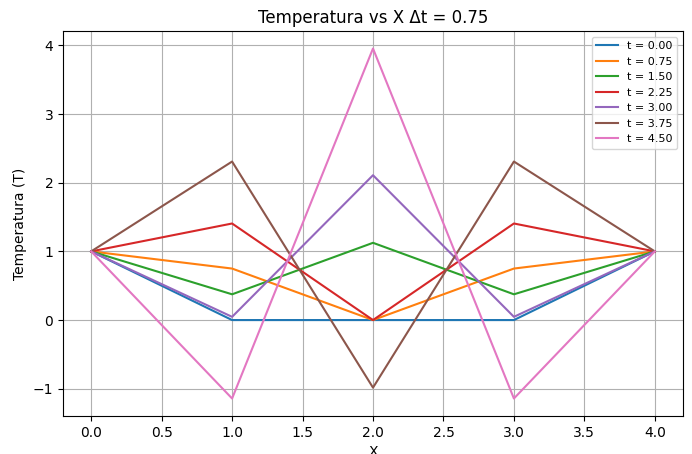
\includegraphics[width=.65\textwidth]{figures/36-3}
	\caption{Temperatura para r=0.75}
\end{figure}


A solução diverge por não atender ao critério de estabilidade de Von Neumann:

\section*{Exercício 3.8}

\subsection*{Solução analítica}

Equação de condução unidimensional com geração

\begin{equation}
	\frac{d^2 T}{dx^2} + \frac{q'''}{k} = 0,
\end{equation}

\begin{equation}
	T(0) = 0, \quad T(L) = 0.
\end{equation}


Uma integração espacial deve ser feita para encontrar T em função de x. Primera integração:

\begin{equation}
	\frac{dT}{dx} = -\frac{q'''}{k}x + C_1
\end{equation}


Segunda integração 

\begin{equation}
	T(x) = -\frac{q'''}{2k}x^2 + C_1x + C_2
\end{equation}


Usando as condições de contorno

Em \(x = 0\):

\[
T(0) = 0 \implies C_2 = 0.
\]

En \(x = L\):
\[
T(L) = 0 \implies 0 = -\frac{q'''}{2k}L^2 + C_1L.
\]

\[
C_1 = \frac{q'''}{2k}L.
\]

Sustituindo obtemos:
\begin{equation}
	T(x) = -\frac{q'''}{2k}x^2 + \frac{q'''}{2}Lx
\end{equation}

\begin{equation}
	T(x) = \frac{q'''}{2k}x(L - x).
\end{equation}


Usando os valores de>
\[
\frac{q'''}{k} = 5 \,{K/m^{2}} ; \quad L = 1 \, m
\]

Obtemos:

\begin{equation}
	T(x) = \frac{5}{2}x(1 - x).
\end{equation}

\subsection*{Solução Diferencias Finitas}

Os cálculos numéricos serão baseados no seguinte esquema do livro do Professor Maliska

\begin{figure}[h]
	\centering
	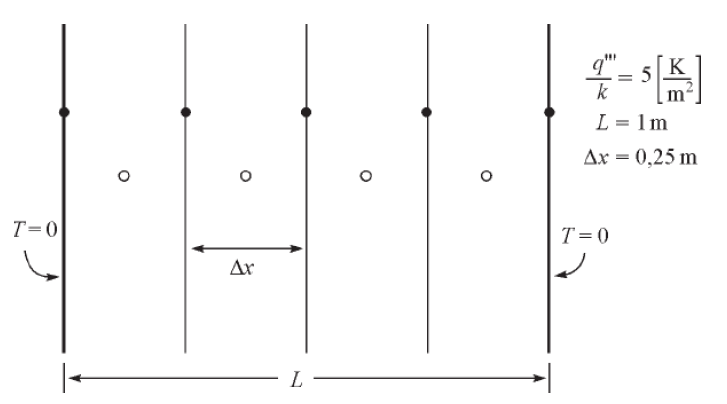
\includegraphics[width=.65\textwidth]{figures/38-1}
	\caption{Solução de condução 1D - Condições de contorno e dados}
\end{figure}

Aproximando a segunda derivada

\begin{equation}
	\frac{\partial T}{\partial x^{2}} = \frac{T_E - 2T_p +T_W}{\Delta x^{2}}
\end{equation}\\
\begin{equation}
	\frac{T_E - 2T_p +T_W}{\Delta x^{2}} + \frac{q'''}{k} = 0
\end{equation}\\

\begin{equation}
	T_E - 2T_p +T_W = - \frac{q'''}{k}\Delta x^{2}
\end{equation} \\

\begin{equation}
	2T_p = \frac{q'''}{k}\Delta x^{2} +T_W +T_E
\end{equation}

Agora comparando graficamente a solução analítica com a solução de diferenças finitas, que foi encontrada resolvendo o sistema linear de equações gerado com o cálculo da equação 37 em cada ponto.

\begin{figure}[H]
	\centering
	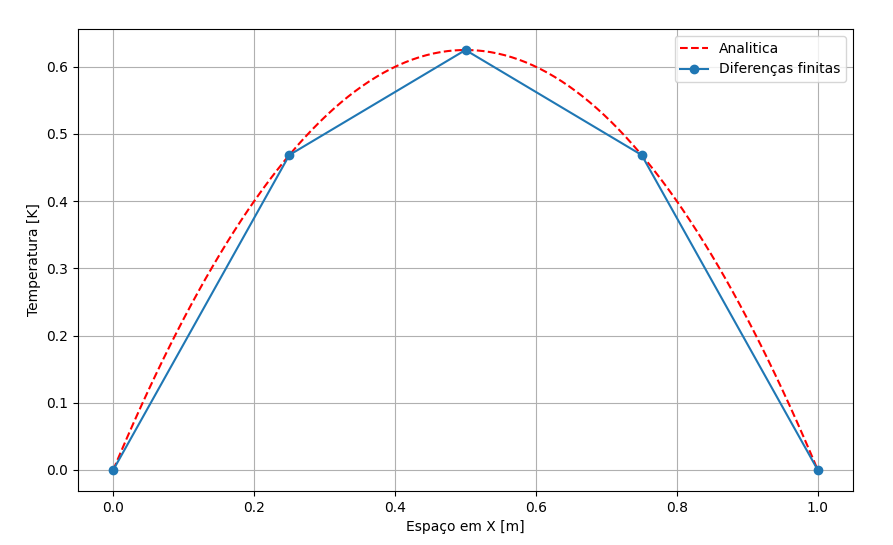
\includegraphics[width=.65\textwidth]{figures/38-2}
	\caption{Solução de condução 1D - forma analítica e diferenças finitas}
\end{figure}


A solução de diferenças finitas reproduz a solução exata, para este caso onde a função de interpolação temporal é utilizada em um problema de regime permanente.


\subsection*{Solução Volumes Finitos}

Usando a equação (37) para encontrar as temperaturas médias nos volumes de controle (conforme indicado pelos círculos brancos), adicionando o balanco nas com interpolação linear de fluxo nas fronteiras esquerda e direita.\\
La interpola
Os resultados para $\delta x = 0.25$ são comparados a soluções que possuem mais volumes de controle

\begin{figure}[H]
	\centering
	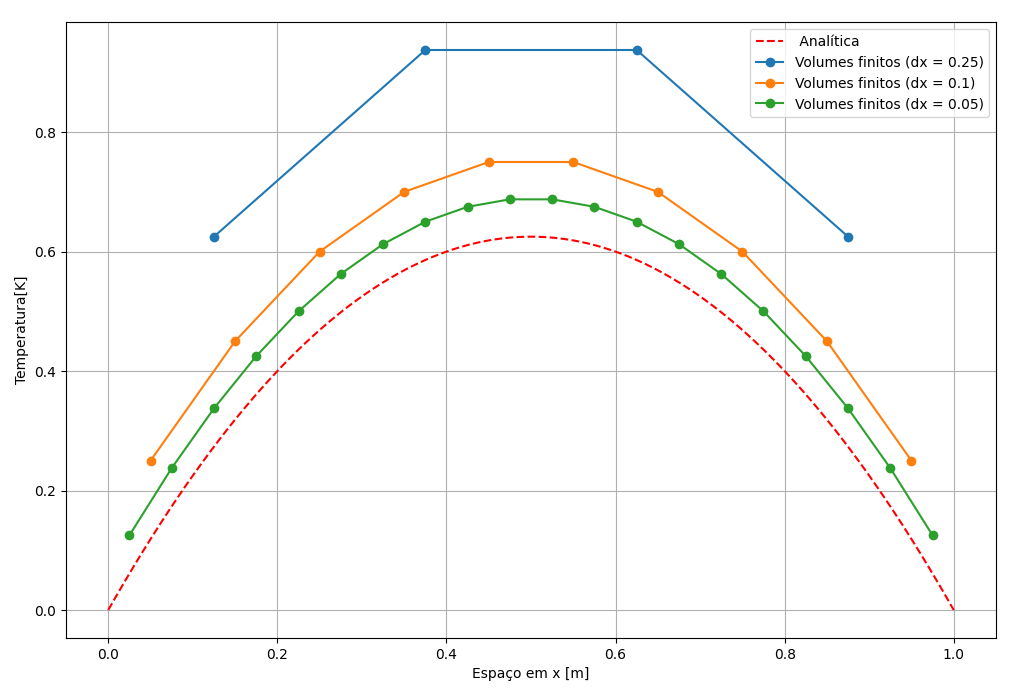
\includegraphics[width=.65\textwidth]{figures/38-3}
	\caption{Solução de condução 1D - forma analítica e volumes finitos}
\end{figure}

Esta figura mostra a dependência da malha para o caso de volumes finitos. Erros de truncamento causam uma diferença na solicitação exata. Discretizações mais finas, como pode ser visto na figura, podem aproximar as duas soluções.

\section*{Exercício 3.9}

Considerando a equação transitória 3.148
\begin{equation}
	\frac{\partial}{\partial t} \left( \rho c_p T \right) = \frac{\partial}{\partial x} \left( k \frac{\partial T}{\partial x} \right) + q'''
\end{equation}

\begin{equation}
	\int_t^{t+\Delta t} \int_w^e \frac{\partial}{\partial t} (\rho T) \, dx \, dt =
	\int_t^{t+\Delta t} \int_w^e \frac{\partial}{\partial x} \left( \frac{k}{c_p} \frac{\partial T}{\partial x} \right) \, dx \, dt +
	\int_t^{t+\Delta t} \int_w^e q''' \, dx \, dt
\end{equation}\\

Propondo integração espacial e temporal

\begin{equation}
	\int_w^e \left( \rho T - \rho^o T^o \right) dx =
	\int_t^{t+\Delta t} \left[ \frac{k}{c_p} \frac{\partial T}{\partial x} \bigg|_e - \frac{k}{c_p} \frac{\partial T}{\partial x} \bigg|_w \right] dt +
	\int_t^{t+\Delta t} q''' \Delta x \, dt
\end{equation}\\
Integrando no espaco e calculando o integrando a media reprsentativa dentro do volume

\begin{equation}
	M_P T_P - M_P^o T_P^o =
	\int_t^{t+\Delta t} \left[ \frac{k}{c_p} \frac{\partial T}{\partial x} \bigg|_e - \frac{k}{c_p} \frac{\partial T}{\partial x} \bigg|_w \right] dt +
	\int_t^{t+\Delta t} q''' \Delta x \, dt
\end{equation}
Usando a função de interpolação de tempo

\begin{equation}
	M_P T_P - M_P^o T_P^o =
	\left[ \frac{k}{c_p} \frac{\partial T}{\partial x} \bigg|_e - \frac{k}{c_p} \frac{\partial T}{\partial x} \bigg|_w \right] \Delta t +
	q''' \Delta x \Delta t
\end{equation}
Usando uma interpolação espacial do forma

\begin{equation}
	\frac{\partial T}{\partial x} \bigg|_e^\theta = \frac{T_E^\theta - T_P^\theta}{\Delta x_e}
\end{equation}

E obtido

\begin{equation}
	\frac{M_P T_P - M_P^o T_P^o}{\Delta t} =
	\frac{k}{c_p} \bigg|_e \frac{T_E^\theta - T_P^\theta}{\Delta x_e} -
	\frac{k}{c_p} \bigg|_w \frac{T_P^\theta - T_W^\theta}{\Delta x_w} + q'''  \Delta x \Delta t 
\end{equation}

Definindo a função de interpolação

\begin{equation}
	T^\theta = \theta T + (1 - \theta) T^o
\end{equation}

Agora, para o \textbf{caso Explicito} $\theta = 0$

\begin{equation}
	\frac{M_P T_P - M_P^o T_P^o}{\Delta t} =
	\frac{k}{c_p} \bigg|_e \frac{T_E^ 0 - T_P^ 0}{\Delta x_e} -
	\frac{k}{c_p} \bigg|_w \frac{T_P^ 0 - T_W^ 0}{\Delta x_w} + q'''  \Delta x \Delta t 
\end{equation}

\begin{equation}
	\left( \frac{M_P c_P}{\Delta t} \right) T_P =
	\left( \frac{k}{\Delta x} \right) T_E^0 +
	\left( \frac{k}{\Delta x} \right) T_W^0 +
	\left( \frac{M_P^o c_P}{\Delta t} - 2 \frac{k}{\Delta x} \right) T_P^o +
	q'' \Delta x
\end{equation}

\begin{equation}
	A_P T_P = A_E T_E^o + A_W T_W^o + \left( A_P^o - A_E - A_W \right) T_P^o + q''' \Delta x
\end{equation}


Aplicando a notação dos coeficientes $A_p, A_NB e A_nb$; e considerando que quando $t\Longrightarrow \infty$ se chega à solução do regime permanente (incluindo a  $q'''$ em B)

\begin{equation}
	A_P T_P^{k+1} = \sum \left( A_{NB} T_{NB} ^k \right) + B
\end{equation}\\

A equação 49 corresponde ao método Jacobi, (3,72 pg 52 Maliska)



E para o\textbf{ caso Implicito } $\theta = 1$
\begin{equation}
	\frac{M_P T_P - M_P^o T_P^o}{\Delta t} =
	\frac{k}{c_p} \bigg|_e \frac{T_E - T_P}{\Delta x_e} -
	\frac{k}{c_p} \bigg|_w \frac{T_P - T_W}{\Delta x_w} + q'''  \Delta x \Delta t 
\end{equation}

\begin{equation}
	\left( \frac{M_P c_P}{\Delta t} + 2 \frac{k}{\Delta x} \right) T_P =
	\left( \frac{k}{\Delta x} \right) T_E +
	\left( \frac{k}{\Delta x} \right) T_W +
	\left( \frac{M_P^o c_P}{\Delta t} \right) T_P^o +
	q'' \Delta x
\end{equation}

Ao atualizar as temperaturas calculadas na mesma iteração é possível obter

\begin{equation}
	A_P T_P = A_E T_E^o + A_W T_W + \left( A_P^o - A_E - A_W \right) T_P^o + q''' \Delta x
\end{equation}

\begin{equation}
	A_P T_P = A_W T_W + A_E T_E^0 + B_P
\end{equation}

Implementando a notação usada no caso explícito, verifica-se que a forma é obtida

\begin{equation}
	A_P T_P^{k+1} = \sum \left( A_{NB} T_{NB} ^k+1 \right) AeT^{k}+ B
\end{equation}\\
 
Corresponde ao método de Gauss-Seidel.Se usarmos também a sobrerelaxação da equação 3.149 (Maliska) chegaremos ao método SOR. (equação 3.74 Maliska)


\section*{Exercício 3.10}


 \begin{figure}[H]
 	\centering
 	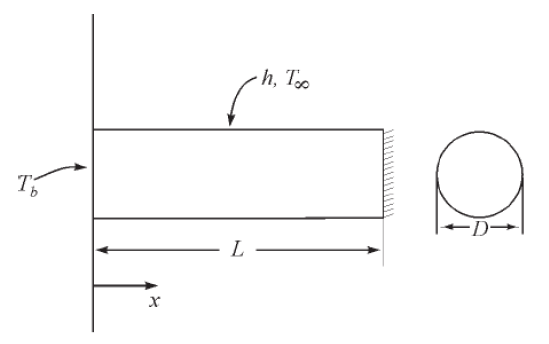
\includegraphics[width=.65\textwidth]{figures/310-1}
 	\caption{O esquema de problema de aleta unidimensional transiente}
 \end{figure}
Tomamos como base a equação do calor de convecção
\begin{equation}
	\frac{\partial^2 T}{\partial x^2} - \frac{hP}{k A_c} (T - T_\infty) = \frac{1}{\alpha} \frac{\partial T}{\partial t}
\end{equation}

Que após a integração temporal e espacial, e usando um esquema implicito,a forma discretizada fica como

'\begin{equation}
	(M_P c_P T_P) - (M_P c_P T_P^0) = \Delta t \left[ \left( k \frac{T_E - T_P}{\Delta x} \right) - \left( k \frac{T_P - T_W}{\Delta x} \right) \right] 
	- \Delta x \Delta t \left[ \frac{hP}{A_c} (T_P - T_\infty) \right]
\end{equation}

\begin{equation}
	T_P \left( \frac{M_P c_P}{\Delta t} + 2 \frac{k}{\Delta x} + \frac{hP}{A_c} \Delta x \right) =
	T_P^0 \left( \frac{M_P c_P}{\Delta t} \right) +
	T_E \left( \frac{k}{\Delta x} \right) +
	T_W \left( \frac{k}{\Delta x} \right) +
	T_\infty \left( \frac{hP}{A_c} \Delta x \right)
\end{equation}

E para um volumen na fronteira livre

\begin{equation}
	T_P \left( \frac{M_P c_P}{2 \Delta t} + \frac{k}{\Delta x} + \frac{hP \Delta x}{2 A_c} \right) =
	T_P^0 \left( \frac{M_P c_P}{2 \Delta t} \right) +
	T_W \left( \frac{k}{\Delta x} \right) +
	T_\infty \left( \frac{hP \Delta x}{2 A_c} \right)
\end{equation}

Resolvendo o sistema de equações pelo método iterativo linha por linha, encontra-se o gráfico a seguir para vários avanços de tempo e sua comparação com a solução analítica. Os resultados sao adimensionales para \\


\begin{equation}
	\theta = \frac{T - T_\infty}{T_{base} - T_\infty} ; x* = \frac{x}{L}
\end{equation}

\begin{figure}[H]
	\centering
	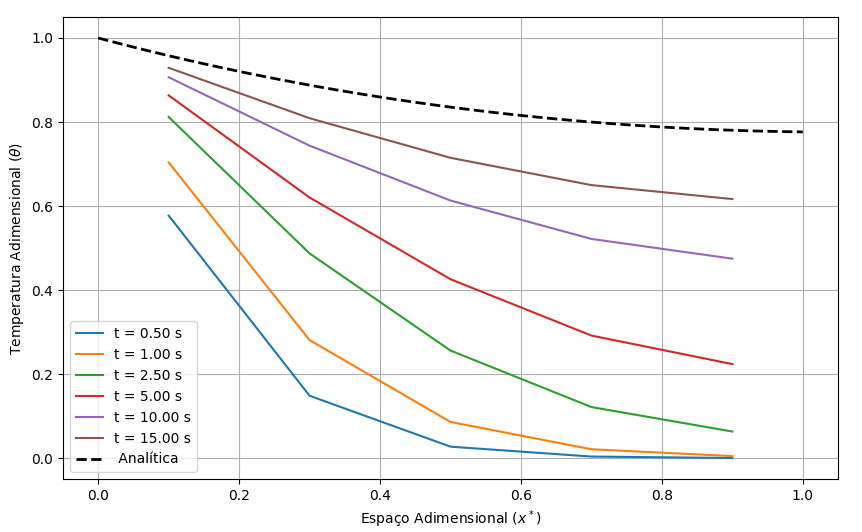
\includegraphics[width=.65\textwidth]{figures/310-2-2}
	\caption{Evolução da temperatura no espaço para 5 volumes de controle}
\end{figure}

Pode-se observar que uma solução numérica de discretização espacial grosseira prevê adequadamente a evolução da temperatura ao longo da aleta. Os diferentes passos de tempo mostram que o regime transiente distorcido quando tende ao infinito alcançará a solução no regime permanente. Um refinamento de malha de 2X mostra um nível de erro mais baixo e uma curva de solução mais contínua conforme esperado.

\begin{figure}[H]
	\centering
	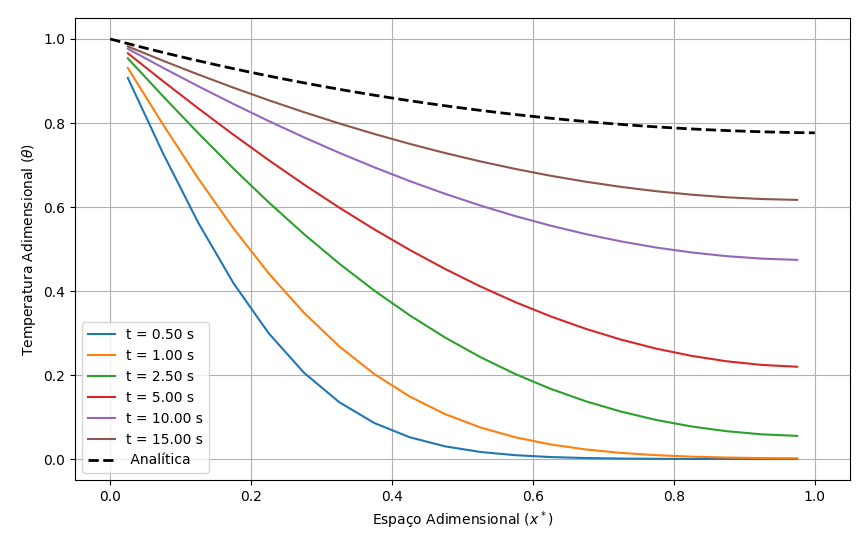
\includegraphics[width=.65\textwidth]{figures/310-3}
	\caption{Evolução da temperatura no espaço para 20 volumes de controle}
\end{figure}


\section*{Exercício 3.16}

começando novamente a partir da equação do calor:

\begin{equation}
	\frac{d^2 T}{dx^2} + \frac{q'''}{k} = 0,
\end{equation}
Integrando no espaço

\begin{equation}
	\int_{w}^{e} \frac{\partial}{\partial x} \left(  \frac{\partial T}{\partial x} \right) dx +
	\int_{w}^{e} \frac{q'''}{k} dx = 0
\end{equation}

\begin{equation}
	 \frac{\partial T}{\partial x} _{e} -
	 \frac{\partial T}{\partial x} _{w}  +
	\frac{q'''}{k} \Delta x = 0
\end{equation}

Organizando os termos e coeficientes

\begin{equation}
	T_P \left( 2 \frac{k}{\Delta x} \right) =
	T_W \left( \frac{k}{\Delta x} \right) +
	T_E \left( \frac{k}{\Delta x} \right) +
	q''' \Delta x
\end{equation}

As expressões para os cálculos de limite serão encontradas eliminando os correspondentes $T_W$ e $T_E$

\subsection*{A}

\begin{equation}
	q''_{entra} + q_{gen} = q_{sai}
\end{equation}
Sustituindo os valores
\begin{equation}
	10 + (7 * 3) \neq 21
\end{equation}

O problema apresenta uma indeterminação devido a um equilíbrio errôneo na equação de energia. O problema com estas condições não tem solução física.

\subsection*{B}
Agora o balanço energético está correto.Para usar o metodo TDMA é necessária uma condição de contorno de Dirichlet para fazer $T_N = Q_N$ e encontrar as variaveis dos pontos $N-1$. Neste caso condições de contorno são fluxos prescritos e não permitem a solução de variáveis para TDMA.\\

Quando a condição de contorno de Dirichlet é usada, o problema fica determinado a resolver os nós internos e a geração.

\subsection*{C}
O problema foi resolvido pelos métodos Jacobi, Gauss-Seidel e SOR. Como esperado, menos iterações são necessárias com o método SOR. As curvas de solução não apresentam diferenças entre os métodos.

\begin{figure}[H]
	\centering
	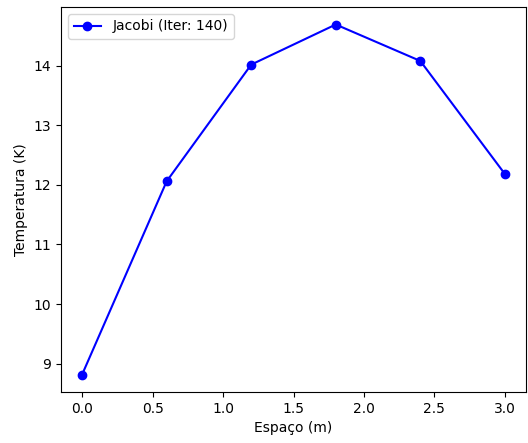
\includegraphics[width=.65\textwidth]{figures/316-1}
	\caption{Evolução da temperatura em relação ao espaço pelo método de Jacobi}
\end{figure}

\begin{figure}[H]
	\centering
	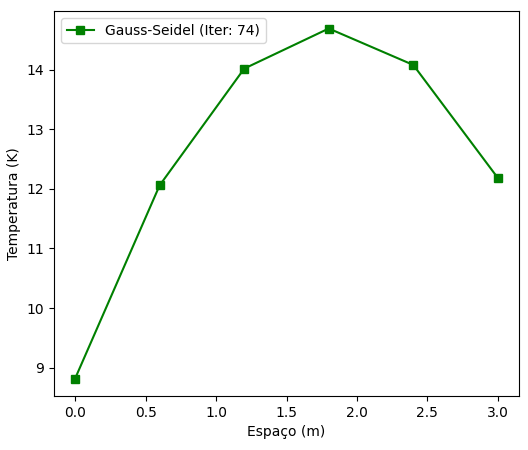
\includegraphics[width=.65\textwidth]{figures/316-2}
	\caption{Evolução da temperatura em relação ao espaço pelo método de Gauss-Seidel}
\end{figure}

\begin{figure}[H]
	\centering
	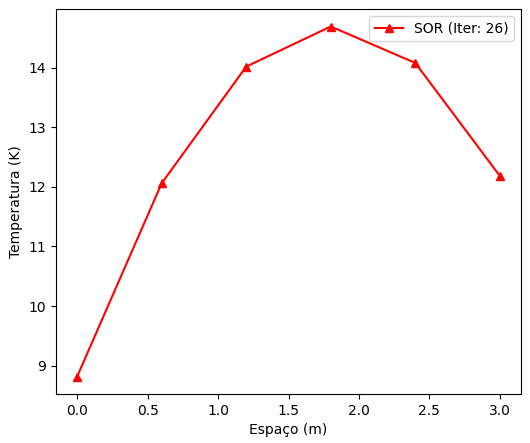
\includegraphics[width=.65\textwidth]{figures/316-3}
	\caption{Evolução da temperatura em relação ao espaço pelo método SOR}
\end{figure}

\section*{Exercício 3.18}
A equação do calor unidimensional em regime permanente é
\begin{equation}
	\frac{d^2 T}{dx^2} = 0
\end{equation}
Com condições do contorno
\begin{equation}
	T(x) = \sin(\pi x) \left( 1 + 0.1 \cdot (-1)^n \right)
\end{equation}
E condiçao inicial $T_{(x=0)}=0 $ e $T_{(x=1)}=0 $\\

Agora discretizando a equação diferencial, como nos exercícios anteriores, temos que

\begin{equation}
	\frac{T_{i+1} - 2T_i + T_{i-1}}{(\Delta x)^2} = 0
\end{equation}
\begin{equation}
	T_i = \frac{T_{i+1} + T_{i-1}}{2}
\end{equation}

Resolviendo numericamente pelo metodo Gauss-Seidel ponto a ponto, para 30 volumenes:

\begin{figure}[H]
	\centering
	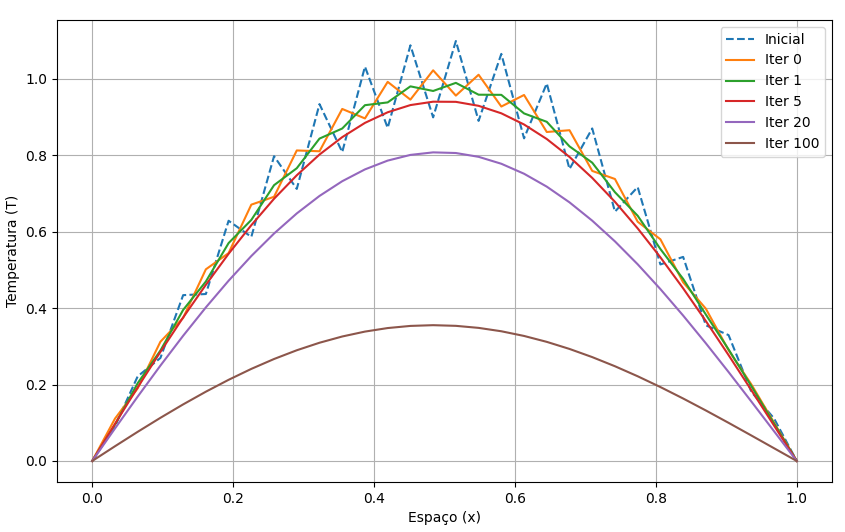
\includegraphics[width=.65\textwidth]{figures/318-1-30N}
	\caption{Evolução da temperatura em relação ao espaço com N=30}
\end{figure}



O gráfico mostra como a temperatura evolui em diferentes momentos da solução (iterações).

\begin{figure}[H]
	\centering
	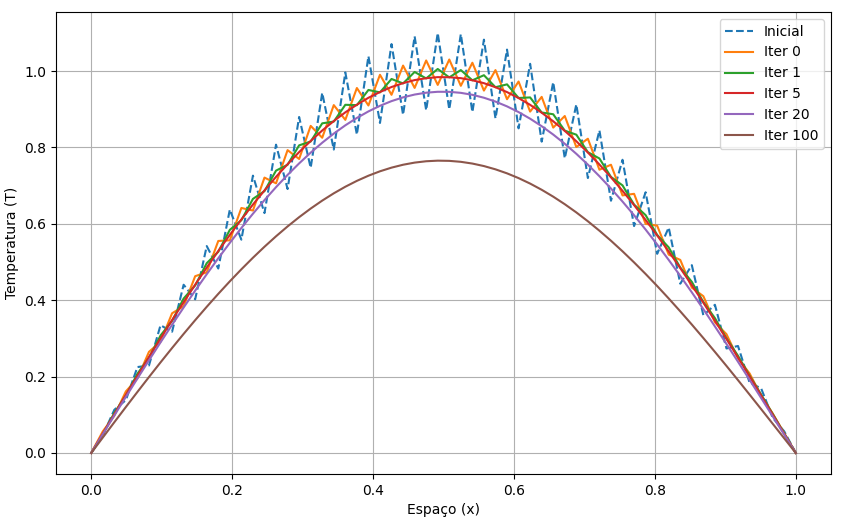
\includegraphics[width=.65\textwidth]{figures/318-1-60N}
	\caption{Evolução da temperatura em relação ao espaço com N=60}
\end{figure}

Com 2X o número de volumes, vemos como a solução nas iterações 20 ou superiores começa a se afastar da solução esperada. Infere-se que à medida que há refinamento da malha, os erros de baixa frequência são mais difíceis de reduzir, consequência da pouca variação de temperatura entre nós adjacentes.

\begin{figure}[H]
	\centering
	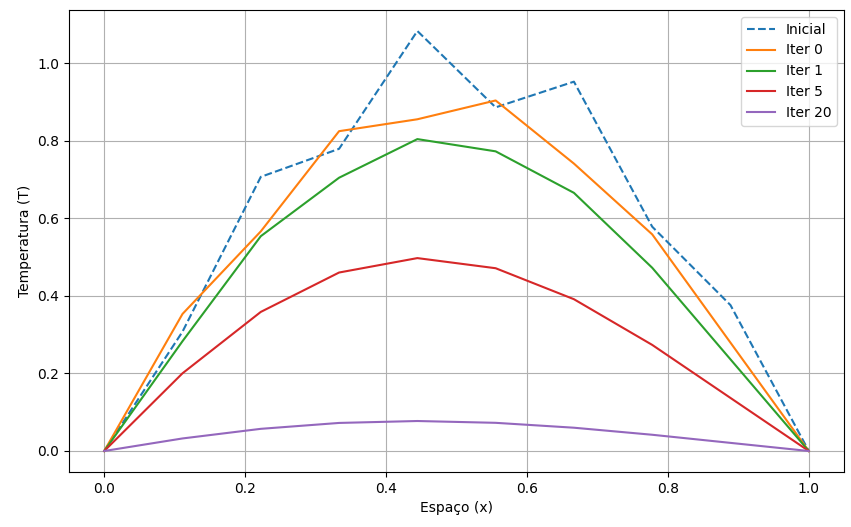
\includegraphics[width=.65\textwidth]{figures/318-1-8N}
	\caption{Evolução da temperatura em relação ao espaço com N=8}
\end{figure}
Levando em consideração os resultados com a malha fina, uma solução com malha grossa mostra como a convergência é alcançada com menos iterações (cerca de 20), implicando que os erros de baixa frequência diminuíram, acelerando a convergência do problema.

\section*{Exercício 2}
\subsection*{A}
\begin{equation}
	A \phi_f + B \frac{\partial \phi}{\partial x} \bigg|_f = C
\end{equation}

\begin{equation}
	 \phi_f= \frac{\phi_p + \phi_w}{2}
\end{equation}

\begin{equation}
	{\frac{\partial\phi}{\partial x}}\bigg|_f =  \frac{\phi_p - \phi_w}{\Delta x}
\end{equation}

Sustituindo

\begin{equation}
	A (\frac{\phi_p + \phi_w}{2}) + B (\frac{\phi_p - \phi_w}{\Delta x}) = C
\end{equation}

\begin{equation}
	\phi_p (\frac{A}{2} + \frac{B}{\Delta x}) + \phi_w (\frac{A}{2} + \frac{B}{\Delta x}) = C
\end{equation}
Organizando

\begin{equation}
	(\frac{A}{2} + \frac{B}{\Delta x}) \phi_p  = (-\frac{A}{2} + \frac{B}{\Delta x}) \phi_w + C
\end{equation}


\subsection*{B}

(i)Valor prescrito 
\begin{equation}
	A \phi_f + B \frac{\partial \phi}{\partial x} \bigg|_f = C
\end{equation}
Para uma condição de contorno de Dirichlet, a derivada espacial é zero.

\begin{equation}
	B \frac{\partial \phi}{\partial x} \bigg|_f = 0
\end{equation}

\begin{equation}
	A \phi_f = C
\end{equation}


\textbf{(ii)Fluxo prescrito}
\begin{equation}
	A \phi_f + B \frac{\partial \phi}{\partial x} \bigg|_f = C
\end{equation}
Na fronteira domina o fluxo, então

\begin{equation}
	A \phi_f = 0
\end{equation}

\begin{equation}
	B \frac{\partial \phi}{\partial x} \bigg|_f = C
\end{equation}
Sim $B=1$\\

\begin{equation}
	\frac{\partial \phi}{\partial x} \bigg|_f = C
\end{equation}


\textbf{(iii)Convecção forçada}

\begin{equation}
	-K\frac{\partial T}{\partial x} = h(T_p - T_{\infty})
\end{equation}

\begin{equation}
	-K\frac{\partial T}{\partial x} = hT_p - hT_{\infty}
\end{equation}
\begin{equation}
	-hT_p + K\frac{\partial T}{\partial x} = hT_{\infty}
\end{equation}


\section*{Exercício 3}

\begin{equation}
	\frac{d^2 T}{dx^2} = 0
\end{equation}
Com distribuição inicial da temperatura
\begin{equation}
	T(x) = \sin(\pi x) \left( 1 + 0.1 \cdot (-1)^n \right)
\end{equation}

E usando a técnica de discretização espacial usada em exercícios anteriores (como 3.6 e 3.8), a evolução da temperatura é representada graficamente para vários números de volumes.
\begin{figure}[H]
	\centering
	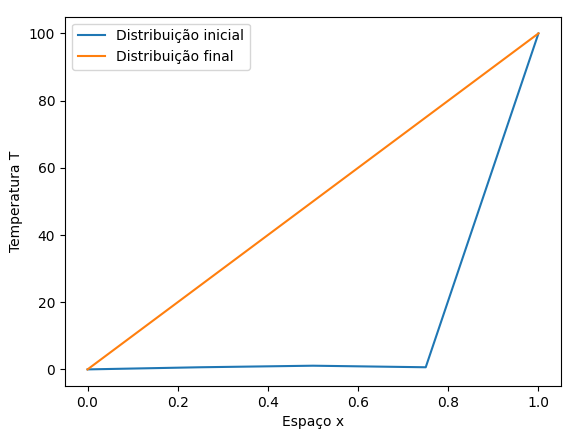
\includegraphics[width=.65\textwidth]{figures/3-2}
	\caption{Evolução da temperatura em relação ao espaço com N=5}
\end{figure}
É possível perceber na figura 16 como durante as primeiras cinco iterações (linha azul) a solução numérica começa a prever a inclinação da solução da equação para regime permanente (que é uma reta). Este caso é para um domínio de 5 volumes.

\begin{figure}[H]
	\centering
	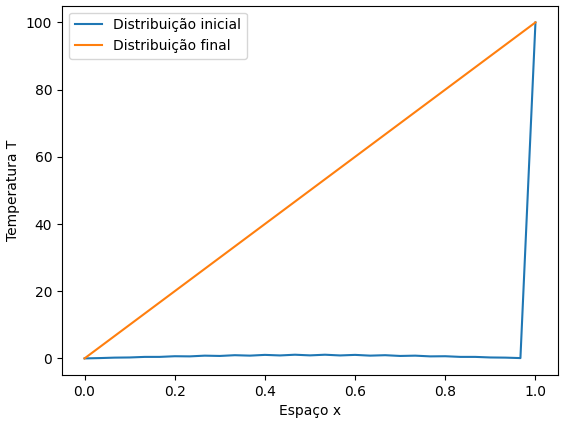
\includegraphics[width=.65\textwidth]{figures/3-3}
	\caption{Evolução da temperatura em relação ao espaço com N=31}
\end{figure}

Com o refinamento da malha, a convergência do problema é mais lenta. A inclinação da curva da distribuição inclinada em relação ao caso de N=5 é maior.

\begin{figure}[H]
	\centering
	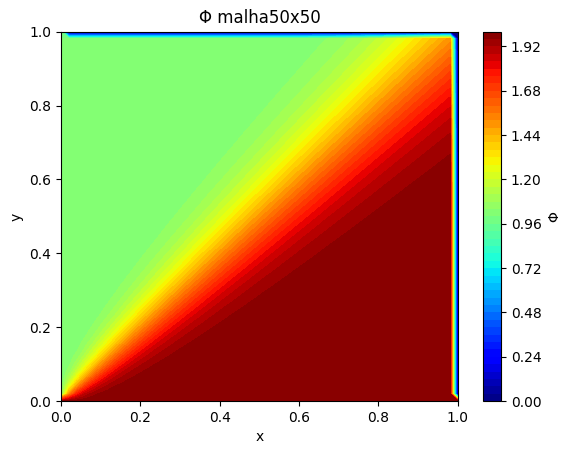
\includegraphics[width=.65\textwidth]{figures/3-4}
	\caption{Comparação dos resíduos máximos para 5, 31 e 101 volumes de controle.}
\end{figure}

\begin{figure}[H]
	\centering
	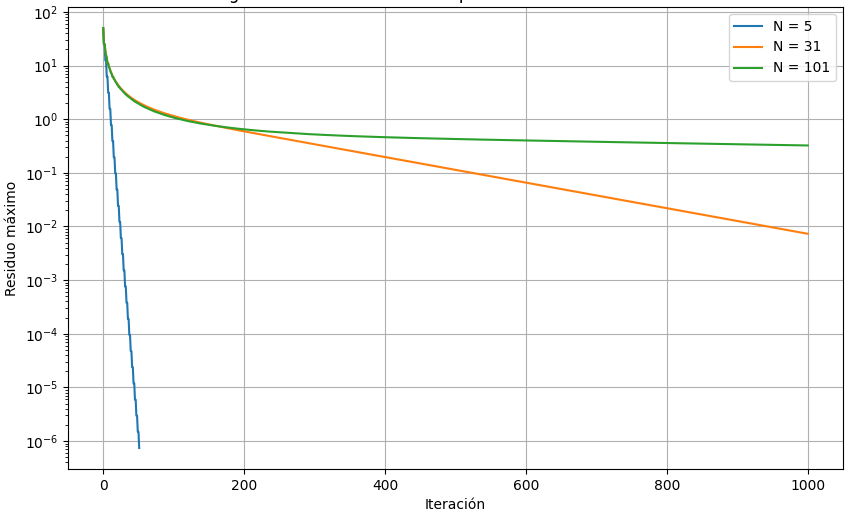
\includegraphics[width=.65\textwidth]{figures/3-1}
	\caption{Comparação dos resíduos máximos para 5, 31 e 101 volumes de controle.}
\end{figure}
A Figura 18 mostra o efeito dos erros de baixa frequência em malhas refinadas. A taxa de convergência diminui com o aumento das colunas de controle. Na Figura 19 podemos ver como esses erros de baixa frequência, devido ao efeito das lentas mudanças de temperatura entre nós vizinhos, impactam na convergência (valor residual em cada iteração). Uma maior velocidade de solução é obtida com a malha mais grossa, mas com menor precisão.

\section*{Exercício 4}
Para a equação de difusão em 2 dimensões com $\alpha = 1$

\begin{equation}
	\frac{\partial T}{\partial t} = 1 \left( \frac{\partial^2 T}{\partial x^2} + \frac{\partial^2 T}{\partial y^2} \right)
\end{equation}\\

Com uma malha não estruturada como neste esquema

\begin{figure}[H]
	\centering
	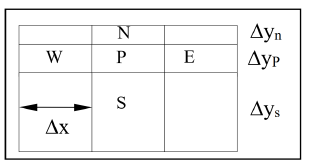
\includegraphics[width=.65\textwidth]{figures/4-2}
	
\end{figure}


O sistema de equações a ser resolvido pode ser inferido com a estrutura seguida nos problemas anteriores, onde para um caso bidimensional a discrtização com diferenças finitas resulta em\\

\begin{equation}
	\frac{T_P - T_P^0}{\Delta t} =
	\left(
	\frac{T_E - 2T_P + T_W}{\Delta x^2} +
	\frac{T_N - 2T_P + T_S}{\Delta y^2}
	\right)
\end{equation}

\begin{equation}
	A_P T_P = A_e T_E + A_w T_W + A_n T_N + A_s T_S + Bp
\end{equation}


Onde

\begin{align*}
	A_P = \frac{\Delta x \Delta y}{\Delta t} + \frac{2 \Delta y}{\Delta x} + \frac{2 \Delta x}{\Delta y} ;A_E = \frac{\Delta y}{\Delta x}; A_W = \frac{\Delta y}{\Delta x};A_N = \frac{\Delta x}{\Delta y}, \quad A_S = \frac{\Delta x}{\Delta y} Bp = T_P^0 \frac{\Delta x \Delta y}{\Delta t}
\end{align*}



	
	\begin{table}[h!]
		\centering
		\begin{tabular}{@{}lcccccc@{}}
			\toprule
			\textbf{Caso} & \textbf{$A_p$} & \textbf{$A_w$} & \textbf{$A_e$} & \textbf{$A_n$} & \textbf{$A_s$} \\ \midrule
			Caso 1        & 5.1            & 1.0            & 1.0            & 2.0            & 0.1            \\
			Caso 2        & 3.2            & 1.0            & 1.0            & 0.1            & 0.1            \\
			Caso 3        & 201.2          & 1.0            & 1.0            & 0.1            & 0.1            \\
			Caso 4        & 23.0           & 1.0            & 1.0            & 10.0           & 10.0           \\ \bottomrule
		\end{tabular}
		\caption{Coeficientes obtidos para cada caso}
		\label{tab:coeficientes}
	\end{table}

A dominância da matriz pode ser estudada com o valor de Ap, que deve ser maior que a soma dos coeficientes dos nós vizinhos para manter a estabilidade numérica. O caso interessante é Caso 3, onde o valor de Ap é muito maior que os coeficientes dos nós adjacentes e torna a matriz muito dominante diagonalmente. Isto é uma consequência do pequeno delta temporal.

Alta anisotropia pode ser observada nos casos 2 e 3 onde os efeitos difusivos são muito maiores na direção x (E e W). Em caso 4 na direção y (S e N).


\section*{Exercício 5}

Da equação de difusão 2D

\begin{equation}
	\frac{\partial^2 \phi}{\partial x^2} + \frac{\partial^2 \phi}{\partial y^2} = 0
\end{equation}

Novamente integrando y discrtizando

\begin{equation}
	\frac{\partial^2 \phi}{\partial x^2} = \frac{\phi_{E} - 2\phi_{P} + \phi_{W}}{\Delta x^2}
\end{equation}

\begin{equation}
	\frac{\partial^2 \phi}{\partial y^2} = \frac{\phi_{N} - 2\phi_{p} + \phi_{S}}{\Delta y^2}
\end{equation}

\begin{equation}
	\frac{\phi_{E} - 2\phi_{P} + \phi_{W}}{\Delta x^2} +
	\frac{\phi_{N} - 2\phi_{P} + \phi_{S}}{\Delta y^2} = 0
\end{equation}

\begin{equation}
	\phi_P = \frac{\alpha (\phi_{E} + \phi_{W}) + (\phi_{N} + \phi_{S})}{2(1 + \frac{\Delta y^{2}}{\Delta x^{2}})}
\end{equation}

\subsection*{A}

Aplicando as condições de contorno para resolver por Gauss Seidel para os casos $\dfrac{\Delta x}{\Delta y} = 1 $ e $\dfrac{\Delta x}{\Delta y} = 10 $, com nivel de erro de 1e-6, obtemos

\begin{figure}[H]
	\centering
	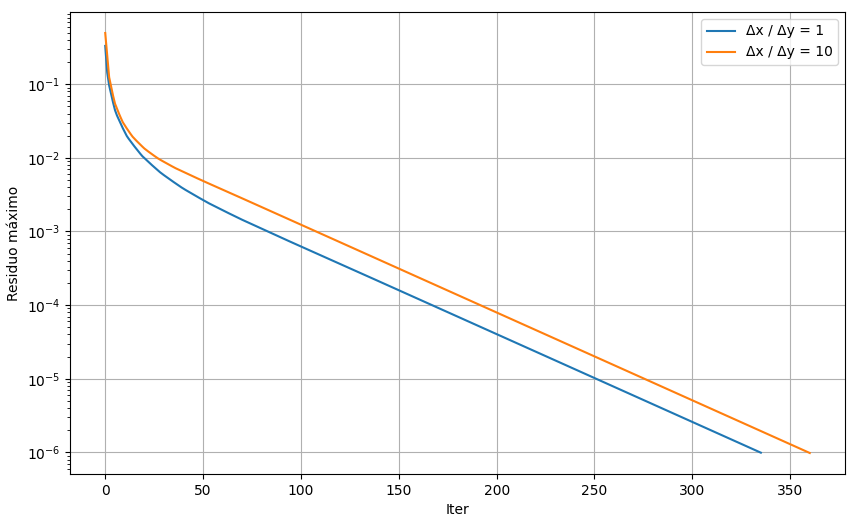
\includegraphics[width=.65\textwidth]{figures/5-1}
	\caption{Comportamento dos resíduos na convergência no caso isotrópico e inosotrópico}
\end{figure}

Menos iterações são obtidas no caso isotrópico. A difusão na direção x ganha importância em relação à difusão em y. Além disso, a condição de contorno na face superior tem impacto na difusão ao longo da direção y negativa.


\subsection*{B}
Agora utilizando TDMA com varreduras em ambas as direções, pode-se notar que este método lida com a anisotropia de forma muito eficiente, resolvendo a varredura horizontal (na direção dominante x) de forma independente e alcançando uma convergência muito mais rápida que o problema isotrópico. No caso isotrópico, o acoplamento entre as cadeias em ambas as direções retarda a convergência e, portanto, requer mais iterações.


\begin{figure}[H]
	\centering
	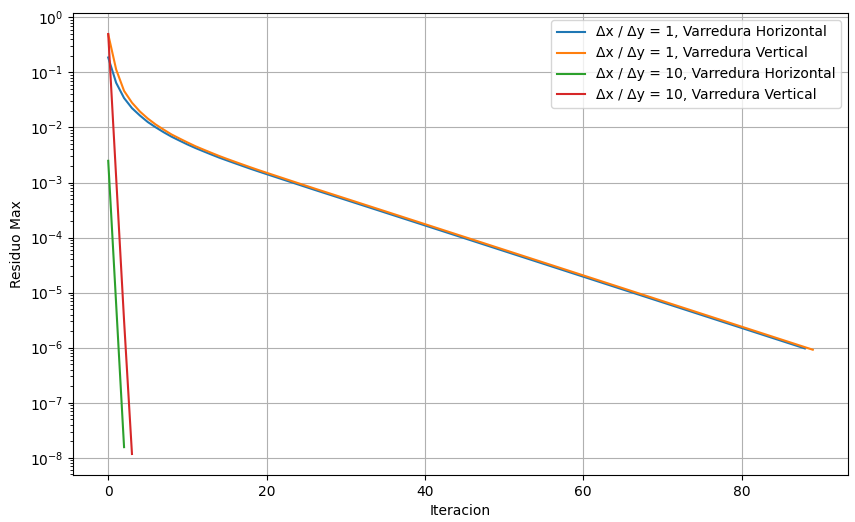
\includegraphics[width=.65\textwidth]{figures/5-2}
	\caption{Comportamento dos resíduos na convergência no caso isotrópico e inosotrópico com TDMA}
\end{figure}




\end{document}





